\chapter[Table of Contents]{Table of Contents (Sumário/Índice)}

O título e o resumo opcional são normalmente seguidos por um índice. Frequentemente você também encontra listas adicionais de ambientes flutuantes, como tabelas e figuras, após o índice (veja a seção 3.20).

Além das opções documentadas nesta seção, os estilos do pacote tocbasic selecionados e configurados com
\verb|\DeclareTOCStyleEntry| (veja a página 387) também têm um impacto significativo na aparência do índice.

Similarmente, os comandos \char`\\\texttt{De\-cla\-re\-Sec\-tion\-Com\-mand}, \char`\\\texttt{Pro\-vi\-de\-Sec\-ti\-on\-Com\-mand}, \char`\\\texttt{Re\-de\-cla\-reSec\-ti\-onCom\-mand} documentados na seção 21.8, página 481 também podem afetar o índice.

O índice é normalmente formatado para que diferentes níveis de comandos de seccionamento tenham recuos diferentes. O número para cada nível é definido justificado à esquerda em um campo de largura fixa. Esta configuração padrão é selecionada com a opção \verb|toc=graduated|.

Se o nível de seccionamento que aparece no índice for muito profundo, o número para esse nível pode ser tão amplo que o espaço reservado para o número é insuficiente. O FAQ alemão [Wik] sugere redefinir o índice em tal caso. O \KOMAScript\ oferece um formato alternativo que evita o problema completamente. Se você usar a opção \verb|toc=flat|, nenhum recuo graduado será aplicado aos títulos dos níveis de seccionamento. Em vez disso, uma organização semelhante a uma tabela é usada, onde todos os números de seccionamento e títulos são definidos em uma coluna justificada à esquerda. O espaço necessário para os números de seção é, portanto, determinado automaticamente.

Você pode encontrar uma visão geral de todos os valores disponíveis para a configuração de \verb|toc| na tabela 3.5.

\begin{figure}
    \centering
    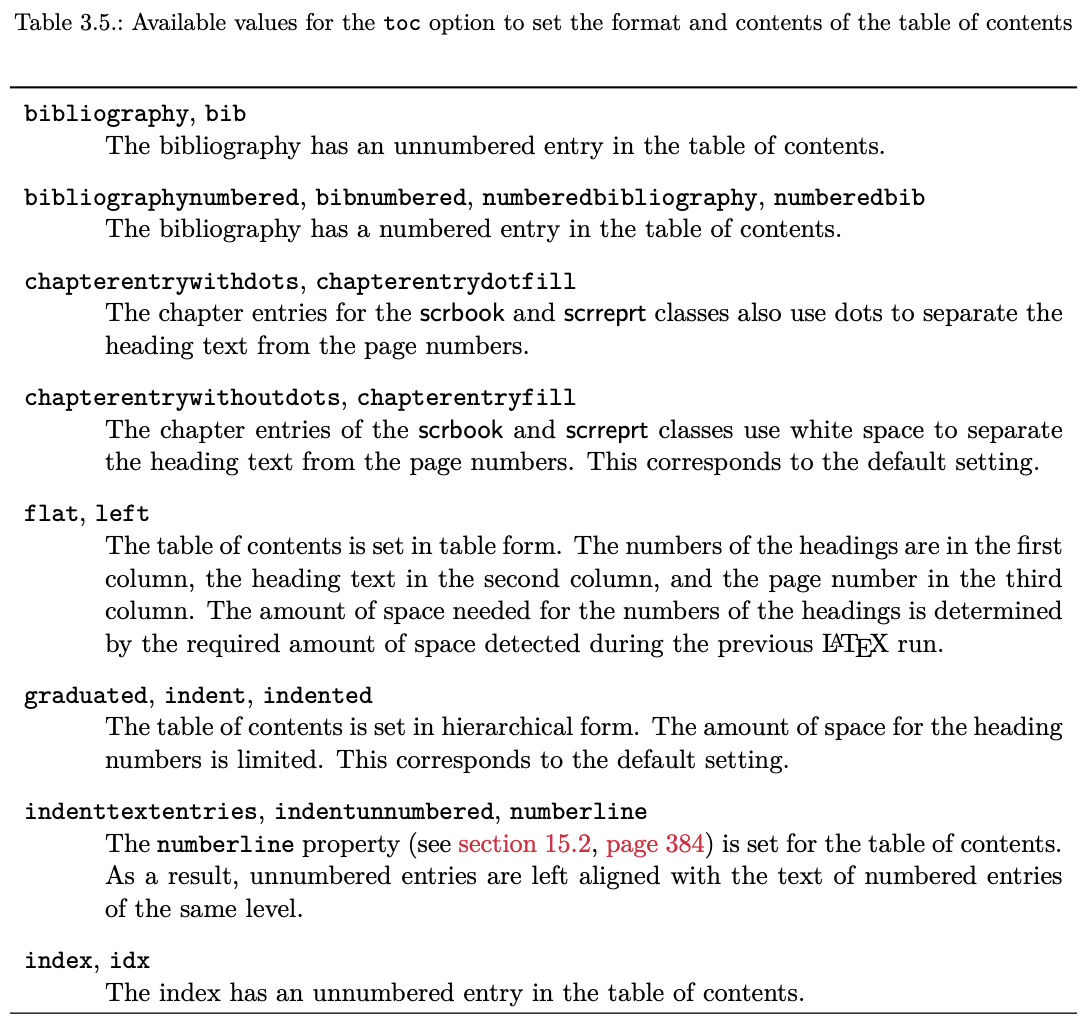
\includegraphics[width=1\linewidth]{imagens/tab3_5.png}
    \caption{Tabela 3.5 do Manual}
    \label{fig:tab3_5}
\end{figure}

\begin{figure}
    \centering
    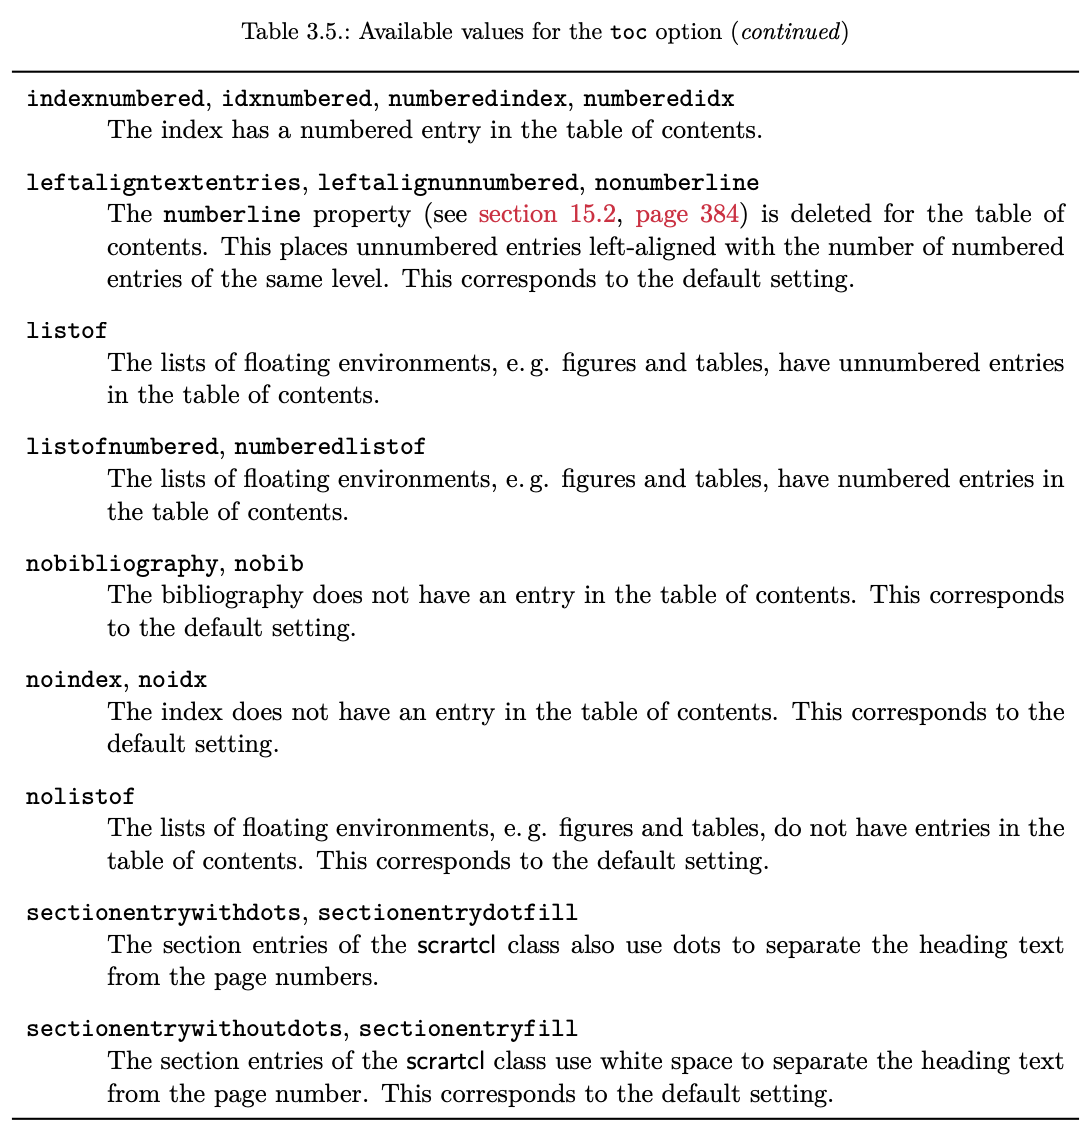
\includegraphics[width=1\linewidth]{imagens/tab3_5b.png}
    \caption{Tabela 3.5 do Manual}
    \label{fig:tab3_5b}
\end{figure}

Normalmente, as divisões de seccionamento incluídas no índice são todas aquelas de \verb|\part| para \verb|\subsection| para as classes scrbook e scrreprt, ou de \verb|\part| para \char`\\\texttt{sub\-sub\-sec\-tion} para a classe scrartcl.

Se deve ou não incluir um nível de seccionamento no índice é controlado pelo contador tocdepth. Ele tem o valor -1 para \verb|\part|, 0 para \verb|\chapter|, e assim por diante. Ao incrementar ou decrementar o contador, você pode escolher o menor nível  de seccionamento para incluir no índice. Aliás, as classes padrão funcionam da mesma forma com as classes padrão, com o \KOMAScript\ você não precisa se lembrar dessas formas. Ao contrário dos valores. O \KOMAScript\ define um comando \verb|\level tocdepth| para cada nível de seccionamento com o valor apropriado que você pode usar para definir \verb|tocdepth|.

Observe que em scrartcl, os valores de \verb|tocdepth| e \verb|secnumdepth| (veja a seção 3.16, página 113) para \verb|\part| não são os mesmos. Esse comportamento foi copiado da classe de artigo padrão para compatibilidade. Assim, por exemplo, você não deve usar \char`\\\texttt{part\-num\-depth} para definir o valor de \verb|tocdepth|.

\textbf{Exemplo}: Suponha que você esteja preparando um artigo que usa o sectioning level \char`\\\texttt{sub\-sub\-section}. No entanto, você não quer que esse nível de \textit{sectioning} apareça no índice. O preâmbulo do seu documento pode conter o seguinte:

\begin{verbatim}
    \documentclass{scrartcl}
    \setcounter{tocdepth}{\subsectiontocdepth}
\end{verbatim}

Assim, você define o contador \verb|tocdepth| para o valor do comando \char`\\\texttt{sub\-sec\-tion\-toc\-depth }. Esse valor normalmente é 2, mas dessa forma, você não precisa se lembrar dele.

Se, em vez disso, você simplesmente quiser incluir um nível a menos no índice do que normalmente faria, você pode simplesmente subtrair um do valor padrão de \verb|tocdepth|:
\begin{verbatim}
    \documentclass{scrartcl}
    \addtocounter{tocdepth}{-1}
\end{verbatim}

O valor que você precisa adicionar ou subtrair de tocdepth é listado no índice de conteúdo após pelo menos duas execuções do \LaTeX.

